\documentclass{article}

\usepackage{amsmath}
\usepackage{amssymb}
\usepackage{graphicx}

\newcommand{\ZZ}{\mathbb{Z}}
\newcommand{\RR}{\mathbb{R}}
\newcommand{\CC}{\mathbb{C}}

\begin{document}

{\bf Worksheet \#19; date: 10/31/2018}

{\bf MATH 55 Discrete Mathematics}

\begin{enumerate}
\item {\em (Rosen 10.3.51)} A simple graph $G$ is called self-complementary if $G$ and $\bar{G}$ are isomorphic. Find a self-complementary simple graph with five vertices.

\item {\em (Rosen 10.3.52)} Show that if $G$ is a self-complementary simple graph with $v$ vertices, then $v \equiv 0$ or $1 \pmod{4}$.

\item {\em (Rosen 10.3.55)} How many nonisomorphic simple graphs are there with five vertices and three edges?

\item Modern K\"onigsberg bridge problem: Was there an Euler path before the bombs? Is there an Euler path after the bombs?
\begin{figure}[htbp]
\centering
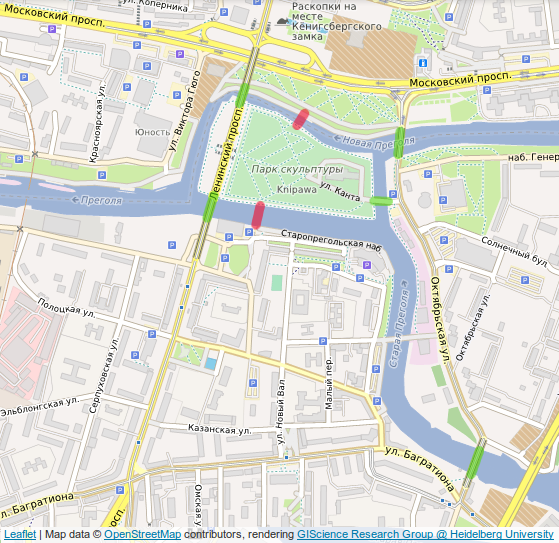
\includegraphics[width=0.6\textwidth]{koenigsberg-current.png}
\end{figure}

\item Suppose a graph has the incidence matrix:
\[
	\begin{pmatrix}
		1 & 1 & 0 & 0 & 0 & 0 & 0 \\
		1 & 0 & 1 & 0 & 0 & 0 & 0 \\
		0 & 1 & 1 & 1 & 0 & 0 & 0 \\
		0 & 0 & 0 & 1 & 1 & 1 & 0 \\
		0 & 0 & 0 & 0 & 1 & 0 & 1 \\
		0 & 0 & 0 & 0 & 0 & 1 & 1
	\end{pmatrix}
\]
More generally, if you know the incidence matrix $A$, how do you check if the graph has a Euler path? What about Euler circuit?

\item {\em (Rosen 10.5.28b)} For which values of $m$ and $n$ does the complete bipartite graph $K_{m,n}$ have an Euler path?

\item Show that the Petersen graph has a Hamilton path but no Hamilton circuit.
\end{enumerate}

\end{document}